\documentclass[a4paper, 12pt]{report}
\usepackage[top = 2.54cm, bottom = 2.54cm, left = 2.54cm, right = 2.54cm]{geometry}
\usepackage{graphicx}
\usepackage{enumerate}
\usepackage{amsmath}
\usepackage{verbatim}
\usepackage{fancyhdr}
\usepackage{fixltx2e} % Package for subscripting and superscripting... %
\pagestyle{fancy}
\setlength{\parindent}{0pt}
\lhead{}
\rhead{Group D - Phase 2 Report}
\renewcommand{\headrulewidth}{0.3pt}

\title{Influenza Virus Infection Modeling}
\author{A.~Ambuehl -- \texttt{antonietta.ambuehl@dtc.ox.ac.uk} \and J.~Leem -- \texttt{jinwoo.leem@dtc.ox.ac.uk} \and M.~Lucken -- \texttt{malte.lucken@dtc.ox.ac.uk} \and W.~Smith -- \texttt{william.smith@dtc.ox.ac.uk} \and O.~Thomas -- \texttt{owen.thomas@dtc.ox.ac.uk} \\\\
University of Oxford DTC \\
Rex Richards Building \\
South Parks Road\\
\underline{Oxford, OX1 3QZ, United Kingdom}\\
}

\begin{document}
\maketitle

%% STYLISTIC COMMENTS %%
%
% Please format function names in computer modern (>> "\textt{}") and latin (i.e., etc., via, e.g.) in italic (>> "\textit{}")
% Citations take >> "glim~\cite{paper}" to give proper spacing.
% Acronymns (as with any other object) should not be pluralised using an apostrophe. (so ODEs not ODE's)
% Don't use the regular speechmarks, they are not formatted correctly (so ``speech'  not "speech"')

\chapter{Background and Aims} %Done by Jin
\section{Biological Problem and Previous Work}
The influenza virus is responsible for a variety of diseases, ranging from the common cold to worldwide pandemics like the Bird flu. For the purpose of treating, and ultimately preventing infections from the virus, it would be desirable to generate a model which simulates the course of viral infection in the human respiratory epithelium. By investigating how viruses interfere with the integrity of the epithelium and the amount of time that is required for the immune response to clear the virus, 

Moreover, it would be most ideal if all aspects of human epithelial immunology (\emph{e.g.} interaction of cytokines, effector cells, antibodies, virions, \emph{etc.}) are incorporated into the prospective model. Initially, a model was devised in 2007 which encompasses many of the factors involved in the immune response ~\cite{Hancioglu}, such as:
\begin{enumerate}[a.]
\item Antibodies and their affinity toward the circulating virus,
\item Antigen presentation,
\item Production and clearance of the virus, \emph{etc.}
\end{enumerate}

This original model is a continuum model based on a series of ordinary differential equations (ODEs); it ultimately predicts changes in the population of healthy and infected cells, and levels of the free virus over the course of infection. \\

In 2013, the results of the model have been reproduced by members of Group G by using a series of Matlab and C++ code ~\cite{GroupG}. This computational model has soundly demonstrated the cellular and viral dynamics in a hypothetical infection scenario with considerable accuracy to the data from the original work. This computational model was superb in that, the user has the freedom to customise the duration of simulations and also set the values for 27 parameters, such as viral release rates, antibody maturation and cellular turnover. \\

%\begin{figure}[htb]
%\includegraphics[]{}                       Include a figure from the original model and the new computational model
%\end{figure}

However, having said this, we felt that the computational model showed modest clinical relevance. The model is designed so that the parameters can be tailored to each patient's immune capacity and each virus strain's virulence, but the model only reflects the natural biological response (\emph{i.e.} the adaptive and innate immune responses) to the virus. In contrast, our group felt that incorporating the effects of anti-influenza drugs on the cellular and viral dynamics was a more pragmatic interpretation of the problem. Consequently, this would allow users to see if treatment is a viable option at specific time points, and raise the need for potential changes in treatment regimes (\emph{e.g.} combinatorial therapy of neuraminidase inhibitors). \\

Furthermore, though our group realised that incorporating more user-dependent parameters could generate outputs for a wide variety of biological scenarios, we equally felt that having absolute control over all 27 parameters may yield biologically-irrelevant results. This would especially be the case if users inadvertently use unreasonable parameter values. For instance, the user may decide to use extremely high rate constants for viral infection ($\gamma_{HV}$) which could lead to false negatives of survival against a viral infection. We also felt that the model assumes some level of staticity; for instance, it assumes that the rate constant of virus formation from the infected cell, $\gamma_{HV}$, is the same in every infected cell. In theory, this value is likely to vary on a cell-to-cell basis (provide reference). Hence, in order to introduce a component to reflect the inherent randomness of the system, we have decided to randomise the input parameters with a pseudorandom number generator. Effectively, we wanted to introduce a level of stochasticity which is controllable to some extent, yet random enough to reflect the randomness of the process. \\

Effectively, we propose the following list of changes to the computational model to improve its general biomedical relevance:
\begin{enumerate}
\item Considering the effects of anti-influenza drugs such as Tamiflu and Relenza (neuraminidase inhibitors) on the release capacity of the virus
\item Addition of helper T-cell (T\textsubscript{H} cell) dynamics as they help to form plasma cells, but their role has been omitted in the original and computational models.
\item Pseudorandomisation of select parameters: a select number of parameters can have their initial values defined by the user, but these input values will be used as a seed for a pseudorandom number generator, thus introducing stochasticity. This will be solved by a stochastic differential equation solver.\\
\end{enumerate}

Ultimately, these extensions culminated to a new model as shown in Figure ~\ref{newmodel}:

\begin{figure}[htb]
\label{newmodel}
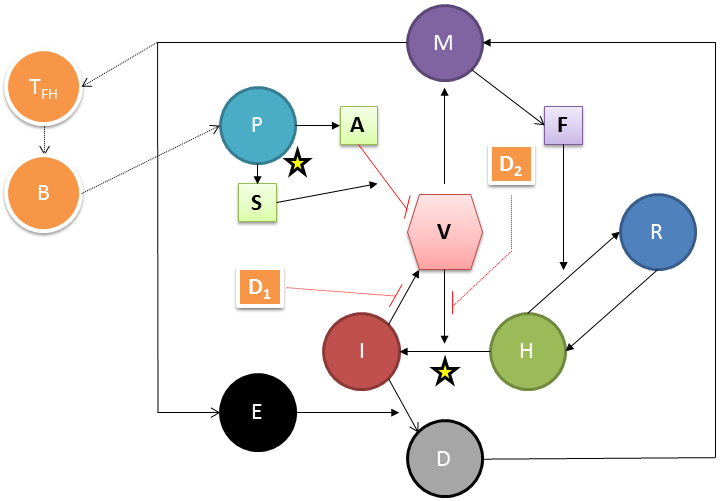
\includegraphics[width = 150mm]{Diagram.png}
\caption{Each of the relevant compartments, as per the original model, are labelled in their respective abbreviations (\emph{e.g.} Infected cells are represented by $I$ and antigen presenting cells (APCs) are represented by $M$, \emph{etc.}). Our additions to the model are labelled as orange compartments with dotted lines for their relevant processes. These new additions include: drugs (neuraminidase inhibitors, $D_1$, and amantadine $D_2$), helper T cell:B cell dynamics (T\textsubscript{FH} and B) and introduction of stochasticity (labelled with yellow stars).}
\end{figure}

\chapter{Extension of the Model}
\section{Modelling Antiviral therapy}
To extend the model, we decided to investigate the effects of adding an antiviral agent to the system.
Antivirals are drugs used to control viral infections both theraputically and prophylactically. They operate by interfering with the virus copying sequence at one or more points in its replication cycle. For example, two common antiviral targets are:
\begin{enumerate}
\item \textbf{Viral M2 proton channels:} Disruption of viral unpackaging in host cytosol \textit{via} the competetive inhibition of the viral M2 proton channel;~\cite{}
\item \textbf{Viral Neuraminidase:} Prevention of viral budding \textit{via} competetive inhibition of the neuraminidases responsible for severing newly-created virus particles from their host cells.\cite{}  
\end{enumerate}
Instances of antivirals exploiting the above mechanisms include Amantadine (trade name ``Symmetrel') and Oseltamivir phosphate (Tamiflu).\\
%Tamifilu works by inhibiting the action of the enzyme viral neuraminidase, whose action is necessary to allow newly-created viral particles to detach from their infected hosts.S
%Symmetrel, an older drug, operates by interfering with the action of viral M2 proton channels, preventing virus particles from becoming decoated once they are absorbed into cells by endocytosis.

Kinetic models have previously been used to investigate the influence of an antiviral drug on viral dynamics within infected individuals. Here we acknowledge the work of Smith and Perelson,~\cite{Smith} who modelled drug influences in simple kinetic models.
The influence of the 2 drug types was accommodated by changing terms in:
\begin{itemize}
\item  $\gamma_HV \rightarrow $ sometheing else TBD
\item $\gamma_V \rightarrow $ sometheing else TBD
\end{itemize}
However, the change assumed a drug concentration that was constant with respect to time. This would have prevented us from analysing effects such as the dependency of drug impact on the drug administration time.
We sought to extend this work by combining a more realistic, temporal drug model with the extended dynamic model of group G. 
Key questions include:
\begin{enumerate}
\item How does the time delay between infection onset and drug administration effect the treatment outcome?
\item Can polytherapy exhibit synergy? \textit{I.e.} could 2 drugs working together ever acheiver more than the sum of their invidudual effects?
\end{enumerate}

\subsubsection{Modelling Viral Drug resistance}

Viruses such as Influenza A are known to be capable of rapidly developing resisitance both to Tamilfu and Symmetrel.
Indeed, innate viral resistance to Symmetrel is now so widespread that it has been withdrawn as a drug.
We sought to model the onset of viral drug resistance by splitting the viral populaton $V$ into subpopulations of different mutants, displaying increasing levels of drug resistance\footnote{The drug resistance was modelled as having an associated fitness cost, making mutation favourable in the presence of antivirals but marginally unfavourable in their absence.}. Initially, all viruses were of an unmutated type, but subsequent mutations (modelled by stochastic population transfers) allow occasional transfer to progressively more resistant types which then proliferate faster owing to the selective pressure imposed by the drug.
%% Are we even including this?

\section{Consideration of T\textsubscript{H} cells in Plasma Cell Dynamics} %By Jin
In the original model, the interaction of T\textsubscript{H}1 and T\textsubscript{H}2 cells were ommitted with almost no justification - this seems unusual, especially considering how critical T\textsubscript{H} cells are fundamental to the clonal expansion of B-cells and their transition into plasma cells. Interestingly, new research suggests that it's neither T\textsubscript{H}1 or T\textsubscript{H}2 cells; instead, another cell type, the follicular helper T-cell, T\textsubscript{FH}, facilitates the switch ~\cite{Swain}. Though it would be ideal to integrate T\textsubscript{FH}:B-cell interaction into the model to enhance its biological relevance, their interaction has not yet been substantially modelled and our group felt it was precocious to propose an entirely new equation to model this interaction. On the other hand, the interaction of T-cells and B-cells has been modelled elsewhere ~\cite{Carneiro1}~\cite{Carneiro2}.\\ 

The change in T-cell population to antigen $k$ (\emph{i.e.} $\frac{dT_k}{dt}$) is dependent on the T-cell death rate ($k_{DT}$), proliferation rate ($k_{PT}$), thymic output rate ($k_{ST}$) and the function $\alpha{T}$ which depends on $\pi_{k}$ (stimulatory signal for T-cell activation), $n_{k}$ (inhibitory signal for T-cell activation), $T_{k}$, and two constants $a_{T1}$ and $a_{T2}$, hence leading to the equation:

\begin{eqnarray}
\frac{dT_k}{dt} &=& -k_{DT} \cdot T_k + k_{PT} \cdot \alpha_{T}(\pi_{k}, n_{k}, T_{k}) + k_{ST}; \label{dTK} \\
\alpha_{T}(\pi_{k}, n_{k}, T_{k}) &=& exp\left[-\left(\frac{log(n_{k}) - a_{T1}}{a_{T2}}\right)^{2}\right]
\end{eqnarray}

The population of active B cells, $B_{i}$, is dependent on the T-cell population; like equation ~\ref{dTK}, $B_{i}$ depends on B-cell death rate ($k_{DB}$), proliferation rate ($k_{PB}$), and the function $\alpha{B}$ (which depends on $\sigma_{i}$ [B cell induction signal], $\tau_{i}$ [number of active T cells], $\beta_{i}$ [the number of induced B cells] and $B_{i}$), thus leading to:
\begin{eqnarray}
\frac{dB_i}{dt} &=& -k_{DB} \cdot B_i + k_{PB} \cdot \alpha_{B}(\sigma_{i}, \tau_{i}, B_{i}); ~\label{dBI} \\
\alpha_{B}(\sigma_{i}, \tau_{i}, B_{i}) &=& \frac{\tau_{i}\cdot{\beta_{i}}}{\tau_{i} + \beta_{i}}, \\
\beta_{i} &=&  exp\left[-\left(\frac{log(\sigma_{i}) - b_{1}}{b_{2}}\right)^{2}\right] \cdot B_{i}
\end{eqnarray}

Surprisingly, for the purposes of analysis, the authors simplify both ~\ref{dTK} and ~\ref{dBI} assuming that there is at least one activated T-cell, thus reducing this system to:
\begin{eqnarray}
\frac{dT_k}{dt} &=& (k_{PT}-k_{DT}) \cdot T_k \\ ~\label{dTKSimple}
\frac{dB_i}{dt} &=& -k_{DB} \cdot B_i + k_{PB} \cdot \frac{T_{k} \cdot B_{i}}{T_{k}+B_{i}}; ~\label{dBISimple}
\end{eqnarray}

Given this new simplified formula, we decided to assimilate these two equations into the existing computational model. Unfortunately, one of the biggest challenges was actually fitting the newly-defined T\textsubscript{FH} cells into the overall scheme in Figure ~\ref{newmodel}. Considering that the mechanism of T\textsubscript{FH} cell differentiation remains undefined and the possibility that T\textsubscript{FH} cells are activated by B cells ~\cite{Crotty}, the equations that we are using may be inaccurate. On the other hand, there is sufficient evidence to suggest that T\textsubscript{FH} cells are activated by signals derived from APCs - thus, continuing with this notion, we suggest that equation ~\ref{dTKSimple} is scaled by the population of APCs, $M$.

\begin{equation}
\frac{dT_k}{dt} = (k_{PT}-k_{DT}) \cdot T_k \cdot M \\
\end{equation}

Under the new scheme, na\"\i ve B-cell activation by T\textsubscript{FH} cells can be represented by equation ~\ref{dBISimple}. As for the subsequent formation of plasma cells from B cells, we can see the original ODE for the formation of plasma cells (where $b_{PM}$ and $\alpha{P}$ are constants representing plasma cell synthesis and death, respectively):
\begin{equation}
\frac{dP}{dt} = b_{PM}MP + \alpha_{P}(1 - P)
\end{equation}

We decided to modify this equation slightly; we retained the constants as they represent properties intrinsic to the \emph{plasma cell}. However, we changed the dependence of plasma cell synthesis to the population of active B cells, $B_{i}$, rather than M (\emph{N.B. }To avoid confusion in nomenclature, $b_{PM}$ was renamed to $b_{PB}$). Therefore, we would attain:
\begin{equation}
\frac{dP}{dt} = b_{PB}B_{i}P + \alpha_{P}(1 - P)
\end{equation}

In summary, to account for the role of helper T cells in plasma cell synthesis with the influenza virus (V) as the antigen, we propose the following system of ODEs:
\begin{eqnarray*}
\frac{dT_V}{dt} &=& (k_{PT}-k_{DT}) \cdot T_V \cdot M \\
\frac{dB_i}{dt} &=& -k_{DB} \cdot B_i + k_{PB} \cdot \frac{T_{V} \cdot B_{i}}{T_{V}+B_{i}} \\
\frac{dP}{dt} &=& b_{PB}B_{i}P + \alpha_{P}(1 - P)
\end{eqnarray*}

\section{Introduction of Stochasticity} %Done by Jin and Owen
To improve the current computational model, we felt that giving the user the freedom to incorporate stochasticity into their analyses was essential. The idea was not to replace the code \emph{per se}, but instead give the user a more realistic account of how cell populations and viral titre can vary over time. There were two possible ways of approaching this problem; it is possible to introduce stochastic noise into either the cell populations or the dynamical rate paramters. Both were explored, and are discussed below.

\subsection{Stochastic Populations}

The study of stochastic differential equations (SDEs) is a widely studied topics in mathematics, with many resources for different algorithms and implementations. The ideal is to solve a differential equation with a well-defined noise function adding a stochastic element over time:

\begin{align}
\frac{\mathrm d X}{\mathrm d t}(t) = \mathrm f (X) + \mathrm g(t)
\end{align}

In the above, $f(X,t)$ is the ``drift function" of the system that would comprise a traditional ODE and $g(t)$ is the component that contributes the stochastic noise with time. It is possible to introduce a traditional finite-difference forward-regression approach, by implementing the Euler-Maruyama method for an SDE, such that:

\begin{align}
X(t+\delta t) = X(t) + (\delta t)\, \mathrm f (X(t)) + \sqrt{ \delta t}\, \mathrm G (X(t))\, \eta \quad \text{such that} \quad \eta \in N(0,1)
\end{align}

Here, $N(0,1)$ is a normal distribution, with a mean of zero and standard deviation of one and $G(X(t))$ is the ``diffusion coefficient'' for our system. Given access to the functions $f(x)$ and $G(X)$ and a normally distributed random number generator, it is possible to solve this iteratively, with each new timestep explicitly using the previous one. This is a simple but reliable implementation, which represents a good method for introducing background noise into the concentrations of various variables in our system.

\subsection{Stochastic Rates}

The next approach, which is possibly more theoretically justifiable, is to allow the parameters of the ODE system to vary stochastically with each call of the function $f(X(T))$. This allows the code to isolate the mechanisms are contributing noise, rather than simply adding some arbitrary amount of stochasticity to the variable each timestep. This method allows for the standard library of ODE solving regression algorithms, since it is the drift function that contributes noise rather than the finite different method itself. It is consequently slightly easier to implement in various languages.

\subsection{Implementation in Matlab}

These two approaches were implemented in two different solver functions: \texttt{sdesolver()} and \texttt{sderatesolver()}, respectively. These resembled the native Matlab solvers, but with an extra input, describing the nature of the diffusion coefficient $G(X(t))$. \texttt{sdesolver()} is handed a two by ten dimensoinal matrix containing the vectors $a$ and $b$, used such that $G(X)=a.$*$X.^b$, elementwise. This gives a wide sampling of potential diffusion functions, allowing for easy sampling of interesting parameter spaces. The second function, \texttt{sderatesolver()}, demands two inputs, which specify the strength of the noise added to the creation of V and S, these being judged to be the processes most likely to realistically exhibit highly stochastic behaviour. A difficulty of implementation involved forcing all variables to remain non--negative: if either the numerical methods or stochastic noise push any variables below zero into an unphysical region of phase space, the variables would quickly and collectively diverge into positives or negative infinities. This was avoided with a simple check and modification.

\section{Results}

We observed several interesting phenomena over the course of exploring parameter and solver configurations for the SDEs. These can be loosely grouped into two classes, thodse of noise propagation and virus resurgence.

\subsection{Noise transferrance}

An interesting question which we addressed is the extent to which noise introduced to one parameter will effect the output of another parameter. Choosing S and V as being test cases, we added noise to each independantly and both together, observing the extent to which this effect the behaviour of other variables. We found that noise added to V became manifest in slight perturbations to the response curves of H, I and M., although the curves were still qualitatively the same objects. Noise added to the variable S had no obvious effect: desite being relatively well--connected in the system of ODEs, the other variables were less effected by perturbations in S. This may be owing to the role of S as a logical variable, ranging from its steady states at zero and one; stochastic variation these may be insignificant compared to the overall logical state of the efficacy.

\subsection{Virus Resurgence}

One dynamically significant effect of adding noise to either the virus population V or the rate of creation of V by infected cells is the occurance of virus resurgence and infection. If the noise introduced is significanly large then the virus population plotted against time will feature more than one spike, representing a reappearance of the virus population in the cell population. I speculate that this is the stochasticity pushing the depleted virus count above a threshold, sparking another wave of infection when the antibody count has fallen sufficiently. This new wave is accompanied by a corresponding rise in antibodies in response, hoping to combat the infection. It is interesting that the subsequent virus and antibody peaks are significantly lower than the first wave's: this can be explained by reference to the antibody efficacy S. This grows every time a new infection appears, describing the cell population's capacity to ``remember'' how to combat the virus, making the virus less successful and demanding less antibody concetration for each wave. These effects can be observed in Figure \ref{resurgance}.

\begin{figure}
\begin{center}
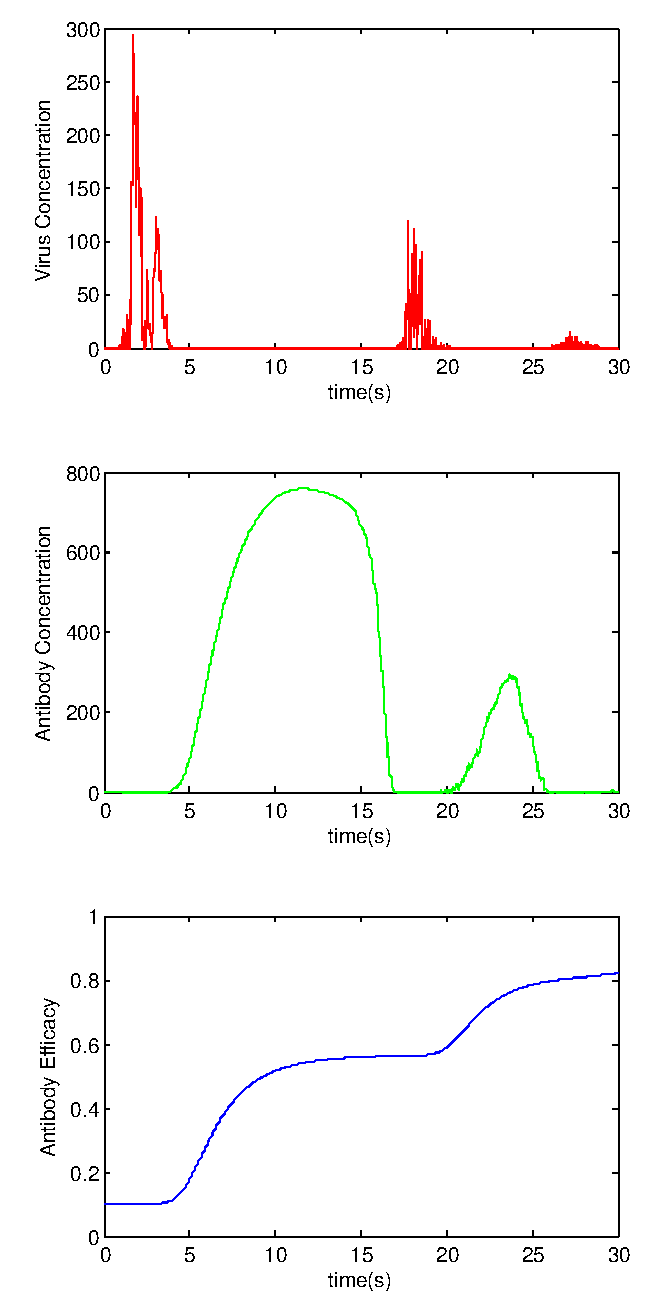
\includegraphics[width=120mm]{Resurgance_scissored.pdf}
\label{resurgance}
\caption{Outputs for V, A and S against time, using the default parameter set and noise on V scaling linearly with V (NoiseParameters(1,1)=NoiseParameters(1,2))}
\end{center}
\end{figure}
%%%% Ignore from here for now
For example, one of the parameters, S (antigenic compatibility of antibodies) is initialised by the user. By using a fixed initial value of antigenic compatibility, \emph{e.g.} $S(0) = x$, we ignore the process of naive B-cell selection (and the possible delay in the immune response due to selection), we also assume that all serum antibodies have affinity $x$ for the virus. In theory, every antibody is constructed from a diverse genetic framework and every antibody has a different affinity for the virus - only the antibody that binds strongest is selected for further expansion in the geminal centres %(provide reference).

% talk about all the changes to the ODEs and why this is mathematically plausible blah blah

% talk about SDE solver and how introducing stochasticity is mathematically plausible blah blah blah

% -Relevance of Stochastic Modeling of the System
% -Explain the use of SDE's
% -Refinement of Code architecture

\chapter{Our code in comparison to Group G}

\bibliography{GroupDReportBibTex}
\bibliographystyle{plain}

\end{document}